\documentclass[../../main.tex]{subfiles}
\begin{document}

{\bf [解]}
円の方程式を$A: x^2+y^2=4$，$B_0: (x-3)^2+y^2=1$とおく．また$B_0$の中心$C_0$，$B$の中心$C$，$A$と$B$の接点を$D$とおく．
$\angle DOC_0=\theta$（$0\le\theta\le2\pi$）の時，$P_0\to P$まで$A$と接していた方の弧長は$2\theta$だから，弧度を含む方の$\angle PCD=2\theta$である．この様子を下図に示す．

\begin{figure}[htb]
\begin{center}
\begin{tikzpicture}[scale=0.9, >=stealth]

  % --- 1. 座標軸 ---
  \draw[->, thick] (-3.5,0) -- (4.5,0) node[right] {$x$};
  \draw[->, thick] (0,-3.5) -- (0,3.5) node[above] {$y$};
  \node[below left] at (0,0) {$O$};

  % --- 2. 大円 A (原点中心, 半径 2) ---
  \draw[thick, blue!80!black] (0,0) circle (2);
  \node[blue!80!black, below left] at (-1.4,-1.4) {$A$};

  % --- 3. 初期状態の円 B_0 (中心 C_0(3,0), 半径 1) ---
  \draw[dashed, gray] (3,0) circle (1);
  \fill[gray] (3,0) circle (1.5pt) node[below] {$C_0$};
  \fill[gray] (2,0) circle (1.5pt) node[below left] {$P_0$};

  % --- 4. 角 theta 回転後の円 B (中心 C, 例: theta = 40度) ---
  \pgfmathsetmacro{\thetaa}{40}
  % C の座標: (3*cos(theta), 3*sin(theta))
  \coordinate (C) at ({3*cos(\thetaa)}, {3*sin(\thetaa)});
  % 接点 D の座標: (2*cos(theta), 2*sin(theta))
  \coordinate (D) at ({2*cos(\thetaa)}, {2*sin(\thetaa)});
  % 点 P の座標: (3*cos(theta) - cos(3*theta), 3*sin(theta) - sin(3*theta))
  \coordinate (P) at ({3*cos(\thetaa) - cos(3*\thetaa)}, {3*sin(\thetaa) - sin(3*\thetaa)});

  % 円 B の描画
  \draw[thick, red!80!black] (C) circle (1);
  \node[red!80!black, above right,yshift=25pt] at (C) {$B$};

  % 補助線
  \draw[dashed, gray] (0,0) -- (C);
  \draw[thick, red!80!black] (C) -- (P);

  % 各点のプロットとラベル
  \fill[black] (D) circle (1.5pt) node[left, font=\small] {$D$};
  \fill[red!80!black] (C) circle (1.5pt) node[above right] {$C$};
  \fill[red!80!black] (P) circle (2pt) node[below right] {$P(X,Y)$};

  % 角度 theta のガイド
  \draw[->, thin] (0.8,0) arc (0:\thetaa:0.8);
  \node[font=\small] at (1.1, 0.3) {$\theta$};

% (ii) 角度 2*theta (角 PCD)
  % CD の方向角は 180 + theta (= 220度)
  % CP の方向角は 180 + 3*theta (= 300度)
  % したがって、角 PCD は 220度 から 300度（差は 2*theta = 80度）
  \pgfmathsetmacro{\startangle}{180 + \thetaa}
  \pgfmathsetmacro{\endangle}{180 + 3*\thetaa}
  
  % C を中心とする半径 0.45 の弧を描画
  \draw[->, thin, red!80!black] ($(C) + ({\startangle}:0.45)$) arc (\startangle:\endangle:0.45);
  % ラベル 2*theta の配置
  \node[font=\small, red!80!black] at ($(C) + ({\startangle + \thetaa}:0.7)$) {$2\theta$};


\end{tikzpicture}
\end{center}
\caption{円 $A$ の周りを転がる円 $B$ と点 $P$ の位置関係}
\end{figure}

この時$\overrightarrow{CP}$の$x$軸からの角度は$\pi-\angle PCD-\angle DOP_0 = \pi-3\theta$で，$P$の座標$P(X,Y)$は
\begin{align}
\begin{pmatrix}X\\Y\end{pmatrix}=\overrightarrow{OC}+\overrightarrow{CP}=3\begin{pmatrix}\cos\theta\\\sin\theta\end{pmatrix}+\begin{pmatrix}\cos(3\theta-\pi)\\\sin(3\theta-\pi)\end{pmatrix}=3\begin{pmatrix}\cos\theta\\sin\theta\end{pmatrix}-\begin{pmatrix}\cos3\theta\\\sin3\theta\end{pmatrix}
\end{align} \label{eq:1}
とかける．この描く曲線がCである．三倍角の公式
\begin{align}
 \begin{cases}
  \sin 3\theta = -4\sin^3\theta + 3\sin \theta \\
  \cos 3\theta =  4\cos^3\theta - 3\cos \theta
 \end{cases}
\end{align}
を代入して
\begin{align}
 \begin{cases}
  X = 6\cos\theta - 4\cos^3\theta \\
  Y = 4\sin^3\theta
 \end{cases} \label{eq:2}
\end{align}
である．


\paragraph{(1)}

\cref{eq:1}のグラフの概形から最大値を求めよう．$X,Y$の一階微分は
\begin{align}
\begin{split}
\dfrac{dX}{d\theta}&=-6\sin\theta + 12\sin\theta\cos^2\theta = 6\sin\theta\left(-1+2\cos^2\theta\right)=6\sin\theta\cos 2\theta \\
\dfrac{dY}{d\theta}&=12\sin^2\theta\cos\theta
\end{split}
\end{align}
だから増減表は下のようになる．ただし$\left.\begin{pmatrix}X\\Y\end{pmatrix}\right|_{\theta=t}$と$\left.\begin{pmatrix}X\\Y\end{pmatrix}\right|_{\theta=2\pi-t}$（$0\le t\le\pi$）が$x$軸に関して対称なので，$0\le\theta\le\pi$とした．

\begin{table}[htb]
  \centering
\caption{曲線$C$の増減表}
\begin{tabular}{c|ccccccccc}
$\theta$ & $0$ & & $\dfrac{\pi}{4}$ & & $\dfrac{\pi}{2}$ & & $\dfrac{3}{4}\pi$ & & $\pi$ \\
\hline
$X'$ & $0$ & $+$ & $0$ & $-$ & $-$ & $-$ & $0$ & $+$ & $0$ \\
\hline
$Y'$ & $0$ & $+$ & $+$ & $+$ & $0$ & $-$ & $-$ & $-$ & $0$ \\
\hline
$(X,Y)$ & $(2,0)$ & $\nearrow$ & $(2\sqrt{2},\sqrt{2})$ & $\nwarrow$ & $(0,4)$ & $\swarrow$ & $(-2\sqrt{2},\sqrt{2})$ & $\searrow$ & $(-2,0)$
\end{tabular}
\end{table}

したがって，$C$（曲線）で$x$座標が最大なのは，$(2\sqrt{2},\pm\sqrt{2})$である．

\begin{figure}[htb]
\begin{center}
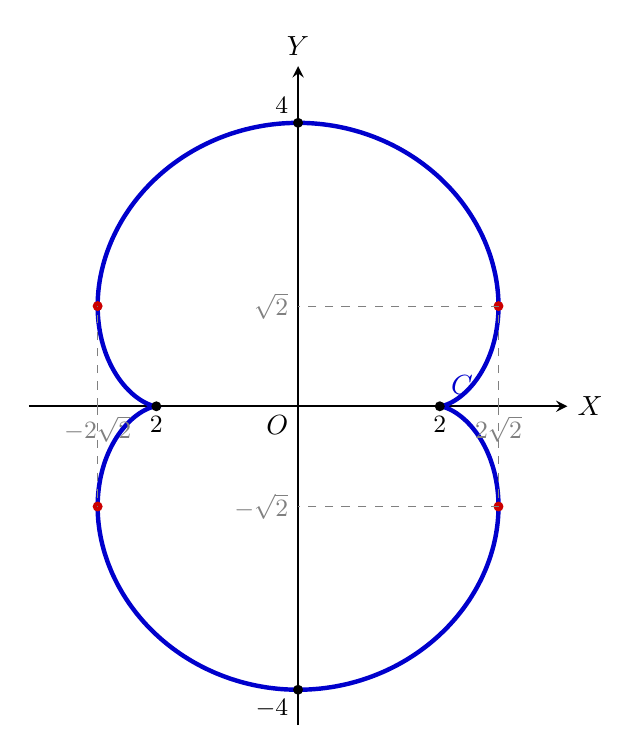
\begin{tikzpicture}[scale=0.9, >=stealth]

  % --- 1. 座標軸 ---
  \draw[->, thick] (-3.8,0) -- (3.8,0) node[right] {$X$};
  \draw[->, thick] (0,-4.5) -- (0,4.8) node[above] {$Y$};
  \node[below left] at (0,0) {$O$};

  % --- 2. 曲線 C の描画 ---
  % X(t) = 3*cos(t) - cos(3*t) = 6*cos(t) - 4*cos^3(t)
  % Y(t) = 3*sin(t) - sin(3*t) = 4*sin^3(t)
  \draw[ultra thick, blue!80!black, domain=0:360, samples=200, smooth] 
    plot ({3*cos(\x) - cos(3*\x)}, {3*sin(\x) - sin(3*\x)}) 
    node[above right] {$C$};

  % --- 3. 増減表で登場する重要な点のプロットとガイド線 ---
  
  % (i) theta = 0, pi, 2pi (X軸上の端点: X = ±2)
  \fill[black] (2,0) circle (2pt) node[below, font=\small] {$2$};
  \fill[black] (-2,0) circle (2pt) node[below, font=\small] {$2$};

  % (ii) theta = pi/2, 3pi/2 (Y軸上の頂点: Y = ±4)
  \fill[black] (0,4) circle (2pt) node[above left, font=\small] {$4$};
  \fill[black] (0,-4) circle (2pt) node[below left, font=\small] {$-4$};

  % (iii) theta = pi/4 (X座標が最大の点: (2sqrt(2), sqrt(2)) ≒ (2.83, 1.41))
  \pgfmathsetmacro{\px}{2*sqrt(2)}
  \pgfmathsetmacro{\py}{sqrt(2)}
  
  \fill[red!80!black] (\px, \py) circle (2pt);
  \draw[dashed, gray] (\px, 0) node[below, font=\small] {$2\sqrt{2}$} -- (\px, \py) -- (0, \py) node[left, font=\small] {$\sqrt{2}$};

  % (iv) theta = 3pi/4 (X座標が最小の点: (-2sqrt(2), sqrt(2)))
  \fill[red!80!black] (-\px, \py) circle (2pt);
  \draw[dashed, gray] (-\px, 0) node[below, font=\small] {$-2\sqrt{2}$} -- (-\px, \py);

  % (v) 第3・第4象限の対称点 (theta = 5pi/4, 7pi/4)
  \fill[red!80!black] (\px, -\py) circle (2pt);
  \fill[red!80!black] (-\px, -\py) circle (2pt);
  \draw[dashed, gray] (\px, 0) -- (\px, -\py) -- (0, -\py) node[left, font=\small] {$-\sqrt{2}$};
  \draw[dashed, gray] (-\px, 0) -- (-\px, -\py);

\end{tikzpicture}
\end{center}
\caption{曲線 $C$の概形と極値点}
\end{figure}

\paragraph{(2)}

$C$の長さを$L$とする．$(X,Y)$が$x$軸についても対称だから，$L$は第一象限の部分の長さの$4$倍である．
したがって
\begin{align}
\begin{split}
\dfrac{L}{4}
 &=\int_0^{\frac{\pi}{2}}\sqrt{\left[3S(2-4S^2)\right]^2+\left[3C(4-4C^2)\right]^2}\,d\theta \\
 &=\int_0^{\frac{\pi}{2}}\sqrt{36S^2(1-2S^2)^2+144C^2S^4}\,d\theta \\
 &=\int_0^{\frac{\pi}{2}}\sqrt{36\sin^2\theta}\,d\theta \\
 &=\int_0^{\frac{\pi}{2}}6\sin\theta\,d\theta \quad(\because\sin\theta\ge0) \\
 &=6\left[-\cos\theta\right]_0^{\frac{\pi}{2}}=6 \\
\therefore
 L&=24
\end{split}
\end{align}
である．

{\bf [解説]}
エピサイクロイドの問題．

\newpage

\end{document}
